\documentclass[12pt]{article}

\title{ECE4063 - Image Thresholding}
%\subtitle{Progress Report}
\author{Emmanuel Jacyna - 24227498 \and James Anastasiou - 23438940}
\date{\today}

\usepackage[T1]{fontenc}
\usepackage[utf8]{inputenc}
\usepackage{rotating}
\usepackage{subfig}

\usepackage{hyperref}
\usepackage{graphicx}
\usepackage{tabularx}
\usepackage{float}
\usepackage{amsmath}
\usepackage{listings}
\bibliographystyle{unsrt}


\begin{document}
\pagestyle{myheadings}
  \maketitle
  \pagebreak
  \tableofcontents
  \pagebreak
  \section{Introduction}
  This document presents our findings and designs for Assignment 2 of ECE4063. It is organised into three major sections, assumptions, solution documentation, and a discussion of potential improvements to the project. Testbench results, Signal Tap results, and RTL diagrams are included in the appendices.\\
  
  The task at hand is to perform binary thresholding on an image for use in a bionic eye. The target platform is an Altera Cyclone II FPGA. In order to threshold the image, a histogram of the pixel greyscale values is calculated and used to find the 50th percentile grey scale value. This value is then used to decide whether to colour pixels white or black, performing an image threshold.
  
  \section{Assumptions}
  When thresholding images, we assume that an image where 99.9\% of pixels are one value is meaningless to threshold. In the case of the Altera DE2 board with Terasic camera module, the small variation in value is likely to be because of pixel noise. We also believe that as the target is a human vision system, 100\% accuracy is not necessarily the goal, as we prefer an image that makes sense to the human eye. This design decision allowed for a simplification of the logic circuit required to determine the most accurate thresholding value. 
  
  We also assumed that Model Sim testbenches are 100\% completely accurate representations of reality. This assumption was routinely called into question, however after fixing a number of other assumptions, this sole assumption was found to be a valid assumption.
  
 
  \section{Documentation - Basic Requirements}
  \subsection{Switch assignments}
  \begin{itemize}
  \item SW[0] -- Displays Touch TCon test vector
  \item SW[1] -- Displays colour image
  \item SW[2] -- Displays greyscale image
  \item SW[3] -- Displays histogram
  \item SW[4] -- Displays cumulative histogram
  \item SW[5] -- Displays simple thresholding
  \item SW[6] -- Displays delayed thresholding
  \item SW[7] -- Displays block thresholding
  \item SW[8] -- Displays interpolated block thresholding
  \end{itemize}
  
  \subsection{RGB to Grayscale conversion}
  There are a number of ways to convert 12bit RGB values into 8Bit Grayscale values, these include taking the average between all 3 colour channels, desaturating the channels or performing a weighted average based on the NTSC standard. Each of these approaches has benefits and weaknesses, our design decision was to approximate the NTSC standard weighted average via fixed shift additions. The decision to approximate the results meant the design did not need to include a multiplier or divider circuit, which significantly improved performance. Three multipliers were replaced with six additions, which if optimised appropriately could utilise Carry Save Adder hardware to improve the performance. Unfortunately as a result of approximating the NTSC values, the actual grayscale values produced to not match exactly with the theoretical values, this was found to be incorrect by a maximum of six units, which we determined to be not a significant loss in precision compared to the speedup and simplification of hardware seen, especially as the end goal of this system is image thresholding.

  \subsection{Total Histogram}
  The Total Histogram is the overall module responsible for managing the histogram generation, cumulative histogram generation, histogram storage and retrieval. This module is implemented as a two-tiered state machine, providing states and certain substates to handle edge cases that arose during testing. This module responds to changes in the frame valid and data valid signals to determine whether to calculate the histogram or the cumulative histogram. It is also able to provide direct read through capabilities, i.e. exposes the histogram RAM interfaces for display purposes.

  \subsubsection{Histogram Module}
  The histogram module provides a wrapper around a single port ram with read while write capabilities. The module is implemented via simple pipelining to minimise the latency of the circuit. The module uses a twenty bit wide RAM with an address bus width of eight bits to store the intermediate results of the histogram. The actual operation of the module is simple, with only a single edge case to handle. This is the case when the same value is read in consecutively. A race condition occurs where an old value is read from the ram before the new value has been written, this is overcome by checking for this condition, and incrementing the registered value by one before writing again, whilst also holding the registered value in a temporary register and checking if the same situation occurs again. By solving this race condition the histogram always produces the correct number of values, and behaves identically to the software (MATLAB) method.\\

  The histogram module also handles clearing its own internal ram, which simplifies the interface for connection to the cumulative histogram module.
  
  \subsubsection{Cumulative Histogram Module}
  The cumulative histogram is significantly more complex than the histogram module, as it is responsible for a number of \textit{administrative} or \textit{house keeping} tasks. The cumulative histogram iterates over the entire contents of the Histogram ram, accumulating the output and storing the result into another RAM for reading by the histogram display modules. While the cumulative histogram module calculates the cumulative sum, it also writes the actual histogram values into one of two RAM's, essentially acting as a double buffered framebuffer. This enables the stored RAM to be used for display on the next frame whilst the new histogram is being calculated. Once the frame is no longer valid, a toggle is switched so that the correct RAM is overwritten with the new values, and the other RAM is kept for display on the next frame.

  \subsection{Thresholding Module}
  \subsubsection{Description}
  The thresholding module is very simple. All it needs to do is take in an eight bit greyscale value and output either a white if the value is above the threshold, or a black if the value is below the threshold. This is accomplished by hooking up a comparator to a multiplexer.
  
  \subsubsection{RTL Diagram}
  \begin{figure}[H]
    \centering{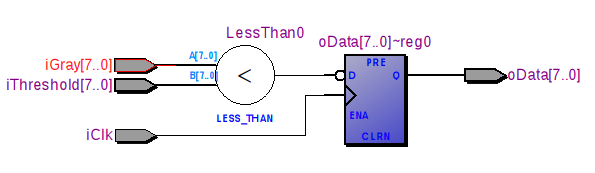
\includegraphics[scale=.8]{Images/ThresholderRTL.png}}
    \caption{Thresholding module RTL}
    \label{fig:thresholder_rtl}
  \end{figure}
  
  
  \subsection{Displaying things}
  \subsubsection{Description}
  In order to display the greyscale image, histogram, cumulative histogram, and thresholded image, we wrote a module to handle multiplexing between them using the switches on the DE2 board, called Arbitrator. This module takes in pixel outputs from the various modules and multiplexes them depending on the switch positions. In order to display images, we simply piggyback on the \(X\_Cont\) and \(Y\_Cont\) signals and modify the \(wr1\_data\) and \(wr2\_data\) inputs to the SDRAM with the appropriate pixel data. \\
      
  Displaying the actual histogram data requires slightly more effort. First we need to extract the histogram data from the histogram RAM and convert the histogram bin contents into lines of appropriate length for display on the screen. To do this we have a module called HistogramDisplayer. This module takes in the \(Y\_Cont\) signal and uses it to index the histogram RAM. Based on the value obtained from the RAM, it scales the histogram value, and uses the \(X\_Cont\) signal to determine the length of the line to be displayed. The decision was made to display the histograms using the full width of the LCD screen. Whilst this does mean that some of the lowest values are not displayed (values less than ten), we found that the lowest black values, due to a quirk of the camera system, never drop below about twelve or thirteen. We thus decided to sacrifice those values in order to get a better view of the histogram as a whole.
  
  \subsection{High Level Overview}
  \begin{figure}[H]
    \centering{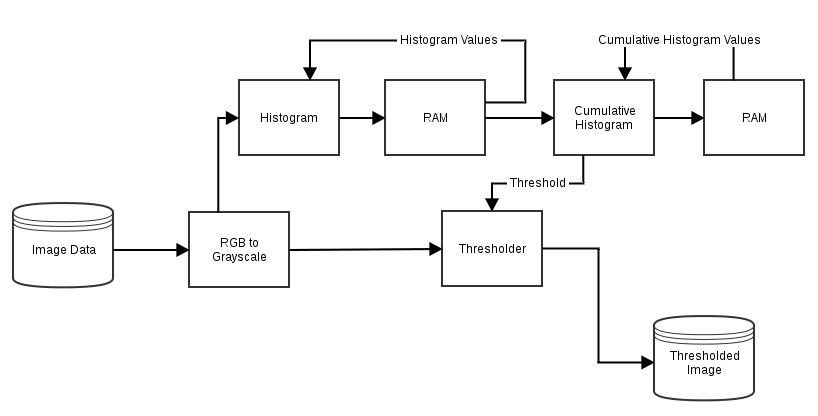
\includegraphics[width=\textwidth]{Images/HistogramOverview.png}}
    \caption{Overview of the image thresholding process}
    \label{fig:histogram_overview}
  \end{figure}
  
  The toplevel module, \texttt{Total\_Module} is fed RGB values from the camera. Those RGB values are then passed through an RGB to greyscale conversion to output greyscale values between 0 and 255. These greyscale values are then passed to the histogram module, which uses an internal RAM to count the number of times each greyscale value is encountered. Once the entire image has been processed, the cumulative histogram module is activated. This module uses its own internal RAM to store the cumulative sum of the histogram. Whilst it calculates the cumulative sum, it checks to see when the cumulative sum passes above the 50th percentile (the point when the sum is less than \(800*480/2\)). It saves this point as the threshold value. On the next frame, this value is then passed through to the thresholder module. The thresholder module uses the threshold it has been given to compare incoming greyscale values to the threshold. Values that are above the threshold are coloured white, and those below are coloured black, thus displaying a thresholded image.
  
  \section{Documentation - Advanced Requirements}
  This section discusses how we approached and achieved the advanced requirements specified in the project.
  
  \subsection{Threshold and Display the Correct Frame}
    \begin{figure}[H]
    \centering{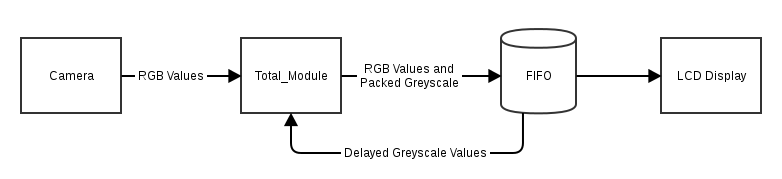
\includegraphics[width=\textwidth]{Images/DelayFrameDiagram.png}}
    \caption{Diagram of delay frame setup}
    \label{fig:hdelyf_ram}
  \end{figure}
  
  In order to successfully threshold the frame the theshold was actually calculated for, we took advantage of the fact that the \(wr1\_data\) and \(wr2\_data\) wires were not fully packed. The data sent to the FIFO buffers consists of three 8 bit RGB values, leaving 8 bits free for us to also send through the grey value. We then recognised that in order to threshold the correct frame, the only information that needs to be delayed that can't be stored on chip was the greyscale values of the image. With this in mind we packed the \(wr1\_data\) and \(wr2\_data\) wires with the relevant grayscale values, resulting in data of the form: texttt{16'bXGGG-GGBB-BBBB-BBXX} and \texttt{16'bXGGG-XXRR-RRRR-RRXX} where \texttt{8'bXXXX-XXXX} is the 8 bit grayscale value, split across the 8 available bits of \(wr1\_data\) and \(wr2\_data\).\\

  When the \texttt{sCCD\_DATA\_VAL} signal goes high, a second read port on the first SDRAM control module reads the data from the FIFO and unpacks the grey value. It then sends the grey value through to the \texttt{Total\_Module} to be thresholded. When the appropriate switch is selected, the arbitrator will output the data from the delayed frame instead of from the current frame. Implementing this frame delaying resulted in a much smoother image on the LCD. This is especially noticeable when rapidly changing the image in front of the camera.

  \subsection{Divided Threshold}
  In order to divide the display into two equal subwindows of half width the \texttt{Y\_Cont} value was used to split the display in half, by a simple comparison with the halfway value of 240, if \texttt{Y\_Cont} was found to be larger than 240, then the larger threshold was used, if it was found to be smaller, then the smaller threshold was to be used. This task only required a small alteration to the \texttt{Cumulative\_Histogram} and \texttt{ThresholdDisplayer} modules, to account for the increased number of threshold values to be generated and used.

  \subsection{Smooth Divided Threshold}
  In order to remove the block artifacts generated by the significant step difference between the two thresholds, the middle 128 (in our final version, actually 256) pixels were thresholded via a linear interpolation between the two thresholds. The step size required to linearly step from threshold two to threshold one was calculated as:
      \begin{equation}
      step = \frac{T2 - T1}{128}
      \end{equation}
  The advantage to using an interpolation window size of 128 is that the division by 128 can instead be achieved by a right shift of 7 bits. However, using this method naively with 8 bit numbers quickly results in very poor interpolation, since the fractional bits disappear when the threshold values are close together. In order to resolve this problem, we left shifted values during calculations, and right shifted them back to the correct magnitude when using them for display.\\
      
  To clarify, we first calculated the delta \(T2 - T1\), then shifted it left by 24 bits to produce a 32 bit number. This provides 24 fractional bits, plenty to work with. We then divided delta by 128 by right shifting it 7 bits. Finally, when stepping through the image, we added the left shifted step size to the left shifted threshold as we progressed along the Y axis, right shifting the resulting threshold back to 8 bits for use in the thresholding module. Using this method allowed us to preserve the fractional bits, helping us to achieve a smooth linear interpolation. In the final product we used a window 256 pixels wide instead of only 128, since the larger window provided a much smoother interpolation effect.

  Our implementation of fractional bits was very inefficient, significant improvements could be found by only shifting left by the absolutely minimum amount needed, the extra bits gained by a shift of 24 instead of 7 (or 8 in our case) provide no extra precision in our use case. The extra bits only serve to slow down that aspect of the circuit, which is a clear example of something that could be easily optimised away.
  
  \section{Acknowledgements}
  We strived to produce only original material, however, we do acknowledge the contributions of others. We obtained some inspiration for the histogram module from a paper published by Maggiani et.al. \cite{histogram}. This paper suggested writing a naive histogram state machine that ignored the consecutive edge case, and instead used multiple histogram cells, essentially independent histograms with indepedent RAMs to hide the RAM access latency and avoid overwriting consecutive values. We did try this method initially, but believed that better use of resources could be obtained by limiting ourselves to one RAM and using a temporary register to handle the consecutive values case. \\
  
  We also obtained ideas from the lectures provided by Dr. David Boland and Dr. Lindsay Kleeman; their suggestions were quite valuable and helped to keep us on track. We also had help from Sam Theodoulou, who gave us a helpful tutorial on the correct usage of Signal Tap.
  
  \section{Improvements}
  There are a large number of improvements we could have made to our project. The first would have been to implement high quality testbenches first. Having excellent testbenches in the last week or so enabled us to rapidly increase our design flow. We could also tidy up the actual Verilog code. There are a few instances of places where we managed to get our design working and left it at that; we didn't want to go changing anything since we had already implemented it correctly. In future it would be better to write cleaner code. \\
  
  Understanding more about the operation of the various top level modules such as the FIFOs and the Touch TCon display would have aided us in completing sooner. It did take a while for us to build a good mental model of the project as a whole.
  
  \bibliography{references}
  
  \newpage
  \section{Appendix A - Testbench Results}
  Testbenching was performed mainly by reading in image data stored in a text file, then writing the results of testbenching to another text file. This was then read in by MATLAB and MATLAB scripts were used to ensure that the testbench result matched the expected result. This appendix provides images of the results obtained from these testbenches.
  \subsection{RGB2GRAY}
    In order to test the \texttt{RGB2GRAY} module, the greyscale conversion, a testbench was written that took as inputs the RGB values of an image, and outputted a file containing the grey values calculated by the modelsim simulation. This was then compared to the MATLAB rgb2gray function results. The mean difference between the MATLAB and Verilog functions was only 6 units, not enough to visibly affect the image output. This was deemed to be well within tolerable bounds. The figures below show the MATLAB image, the Verilog image, and the difference between the two. 
\begin{figure}[H]
  \centering
  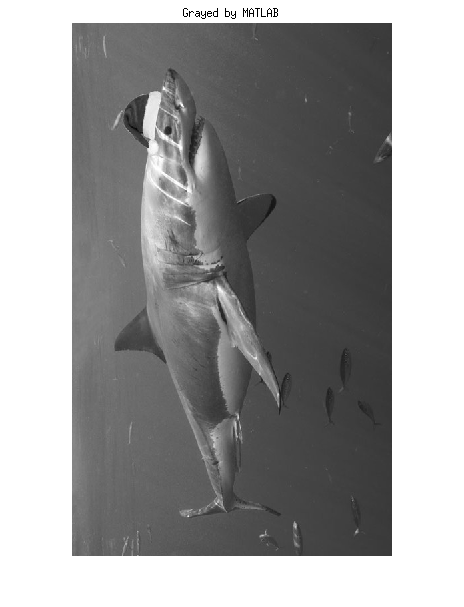
\includegraphics[height=300pt, angle=-90]{Images/RGB2GRAY/MATLAB.png}
  \captionof{figure}{MATLAB rgb2gray result}
\end{figure}

\begin{figure}[H]
  \centering
  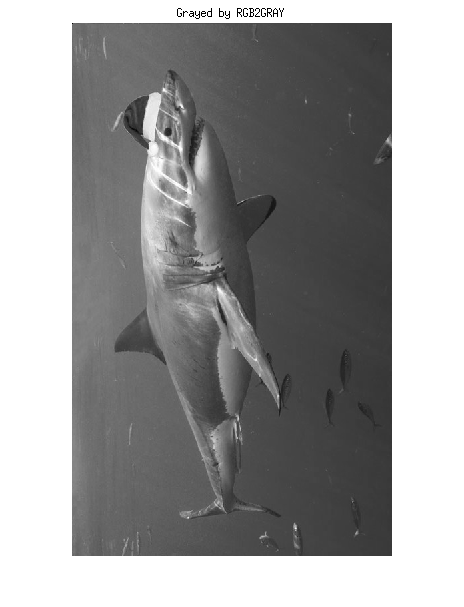
\includegraphics[height=300pt, angle=-90]{Images/RGB2GRAY/Verilog.png}
  \captionof{figure}{RGB2GRAY.v result}
\end{figure}

\begin{figure}[H]
  \centering
  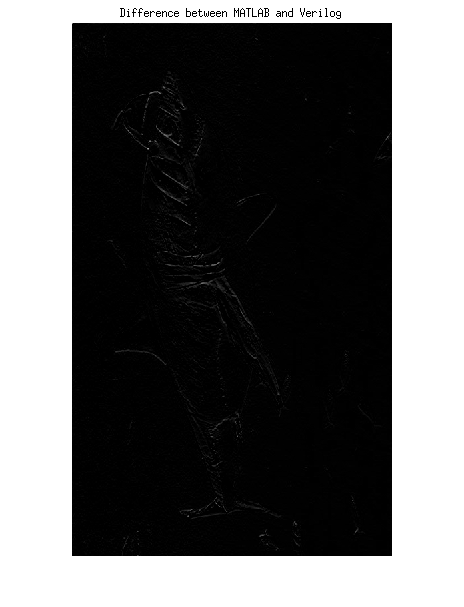
\includegraphics[height=300pt, angle=-90]{Images/RGB2GRAY/Difference.png}
  \captionof{figure}{Difference between the two}
\end{figure}

    
\newpage
  \subsection{Histogram}
  In order to test the \texttt{Histogram} module, a testbench was written to read in precalculated greyscale values and output a histogram. This histogram was then compared to the histogram generated by matlab. The MATLAB code and Verilog code give identical histograms.
  \begin{figure}[H]
    \centering{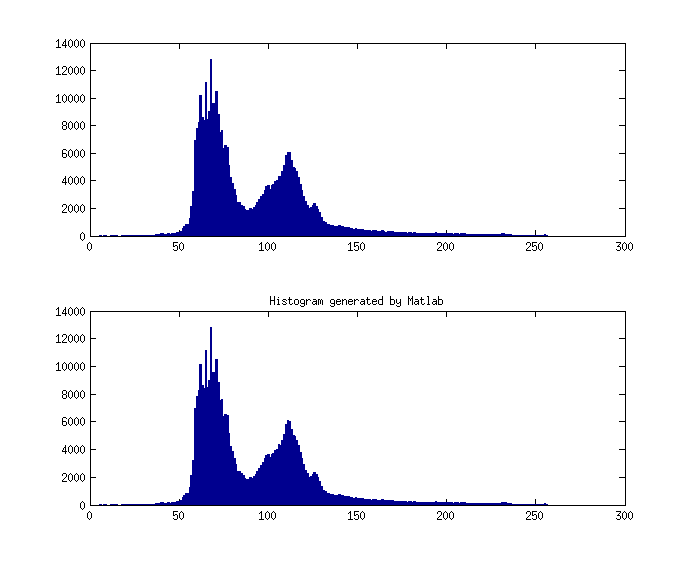
\includegraphics[scale=.8]{Images/HistogramTestbench.png}}
    \caption{Comparison of histogram generated by Histogram module and by matlab}
    \label{fig:histogram_testbench}
  \end{figure} 
  
\newpage
  \subsection{CumulativeHistogram}d
    In order to test the \texttt{CumulativeHistogram} module, a testbench was written to read in a histogram (generated by \texttt{Histogram} module). The cumulative histogram was then calculated and compared to that generated by matlab. The two cumulative histograms are identical.
  \begin{figure}[H]
    \centering{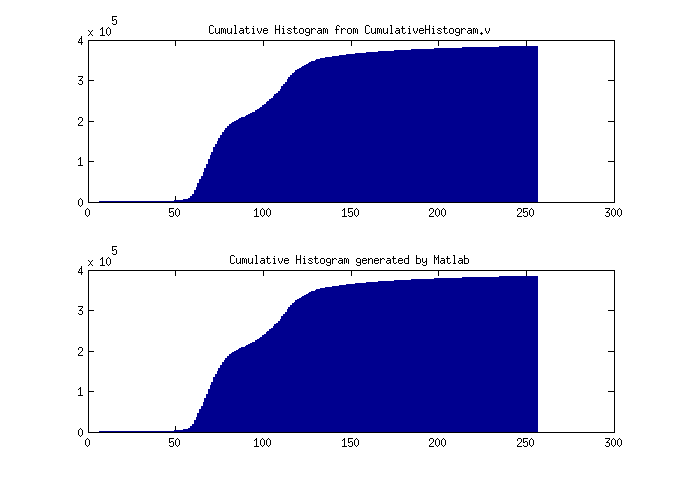
\includegraphics[scale=.8]{Images/CumulativeHistogramTestbench.png}}
    \caption{Comparison of cumulative histogram generated by Cumulative Histogram module and by matlab}
    \label{fig:cumulative_histogram_testbench}
  \end{figure} 
  
\newpage
  \subsection{Total\_Histogram}
    In order to test the \texttt{Total\_Histogram} module, a testbench was written to read in precalculated greyscale values and output a histogram and a cumulated histogram. The result is the same as those calculated with the separate Histogram and CumulativeHistogram testbenches.
  \begin{figure}[H]
    \centering{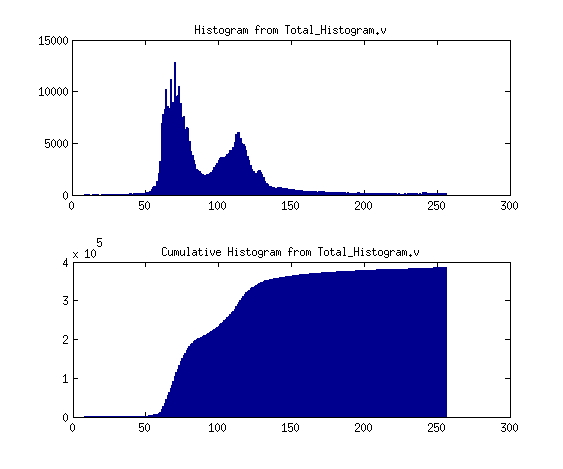
\includegraphics[scale=.8]{Images/Total_HistogramTestbench.png}}
    \caption{Cumulative Histogram and Histogram generated by \texttt{Total\_Histogram} module}
    \label{fig:cumulative_histogram_testbench}
  \end{figure} 
  
\newpage
  \subsection{HistogramDisplayer}
  In order to test the \texttt{HistogramDisplayer} module, a testbench was written to read in histogram values and output the same image that would be outputted on the LCD screen. MATLAB was then used to display the image. The image displayed clearly reflects the histograms displayed above, ignoring normalization.
  \begin{figure}[H]
    \centering{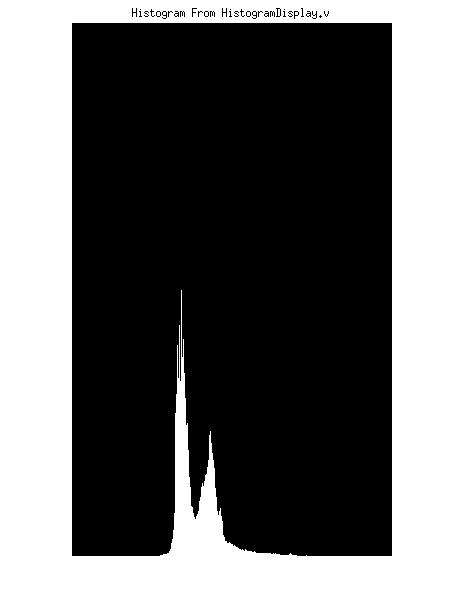
\includegraphics[scale=.8]{Images/HistogramDisplayerTestbench.png}}
    \caption{Image generated by the \texttt{Histogram Displayer module}}
    \label{fig:histogram_displayer_testbench}
  \end{figure} 
  
\newpage
  \subsection{Total\_Module}
  In order to test \texttt{Total\_Module}, we wrote a testbench that reads in RGB values from a file, then passes those through to an instantiation of \texttt{Total\_Module} along with appropriate data valid signals. The testbench then changes the switch settings and outputs image data to file. A matlab script is used to read in this data and display images. The results are below. Clearly the module behaves correctly for the christmas shark input image, confirming our work in simulation.

\begin{table}[h!]
\begin{center}
\begin{tabular} {c c c}
  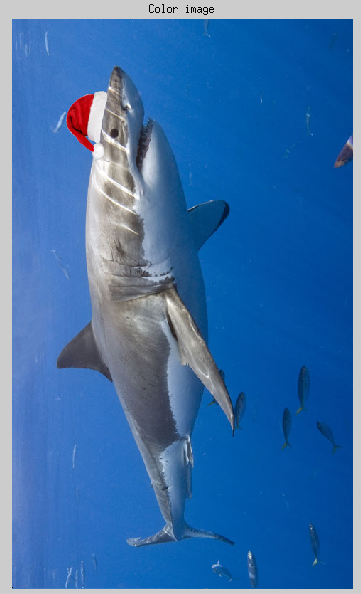
\includegraphics[scale=.52]{Images/TotalModule/RGB.png}
&
  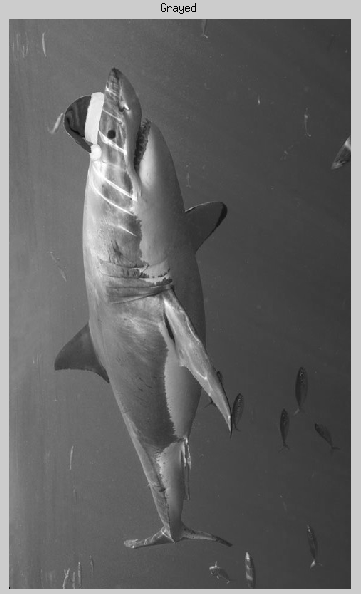
\includegraphics[scale=.52]{Images/TotalModule/Gray.png}
&
  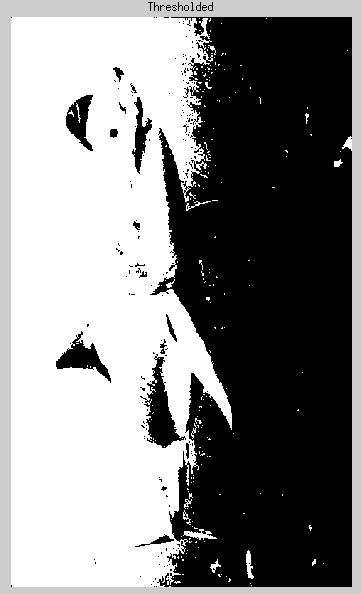
\includegraphics[scale=.52]{Images/TotalModule/Thresholded.png}
\end{tabular}
\end{center}
\captionof{figure}{RGB pass through, grayscale image, and thresholded image}
\end{table}

\newpage
\begin{table}[h!]
\begin{center}
\begin{tabular} {c c}
  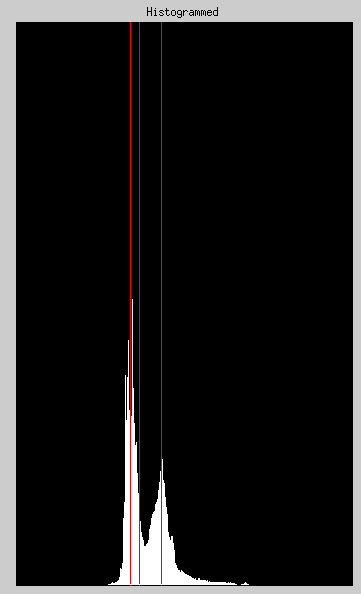
\includegraphics[scale=.8]{Images/TotalModule/Histogrammed.png}
&
  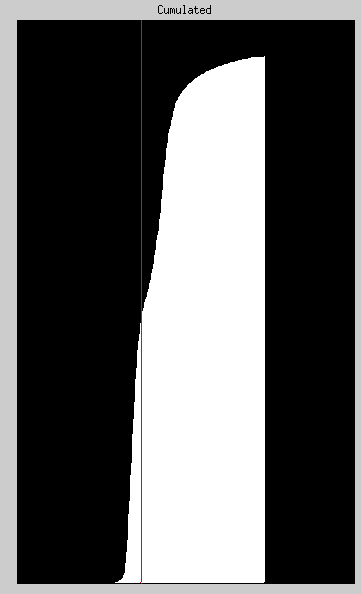
\includegraphics[scale=.8]{Images/TotalModule/Cumulated.png}
\end{tabular}
\end{center}
\captionof{figure}{Histogram and Cumulated Histogram generated by \texttt{Total\_Module}}
\end{table}

\newpage
  \begin{table}[H]
\begin{center}
\begin{tabular} {c c}
  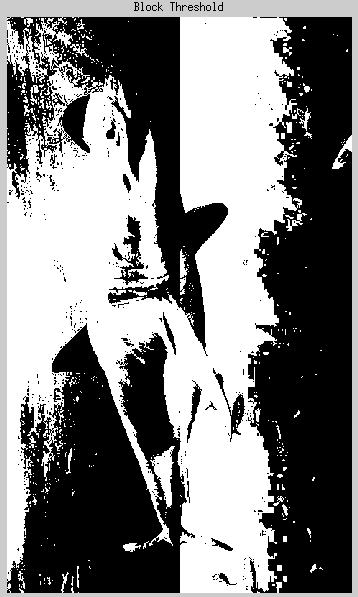
\includegraphics[scale=.8]{Images/TotalModule/BlockThresholded.png}
&
  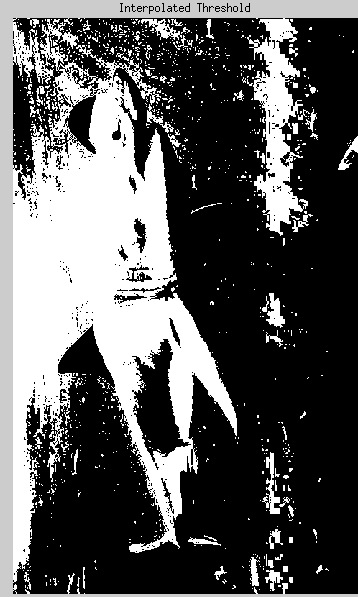
\includegraphics[scale=.8]{Images/TotalModule/SmoothThresholded.png}
\end{tabular}
\end{center}
\captionof{figure}{Block Threshold and Interpolated Threshold generated by \texttt{Total\_Module}}
\end{table}
  
  
\newpage
  \subsection{MultiThresh}
  In order to test the \texttt{MultiThresh} module, a testbench was written to read in greyscale values and run them through the MultiThresh module. After displaying the resulting image data in MATLAB we were able to verify that the module worked correctly.
  \begin{table}[h!]
\begin{center}
\begin{tabular} {c c}
  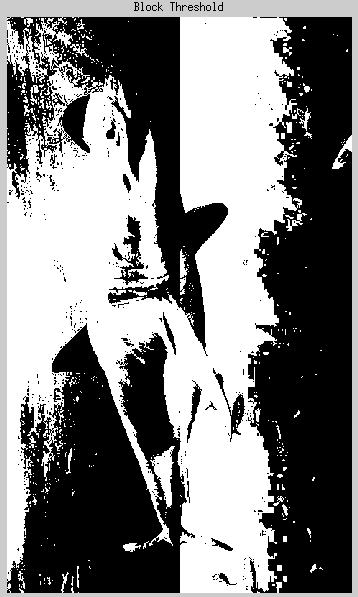
\includegraphics[scale=.6]{Images/TotalModule/BlockThresholded.png}
&
  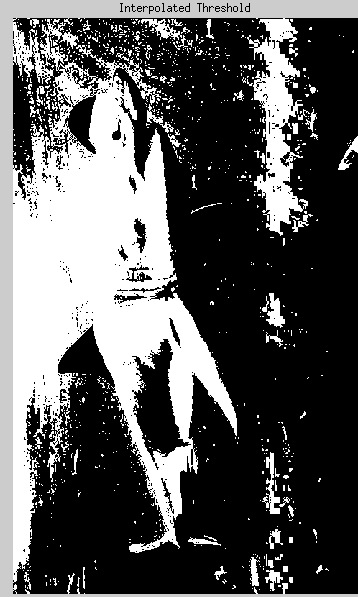
\includegraphics[scale=.6]{Images/TotalModule/SmoothThresholded.png}
\end{tabular}
\end{center}
\captionof{figure}{Block Threshold and Interpolated Threshold generated by \texttt{MultiThresh}}
\end{table}

\newpage
  \subsection{Delayed Frame}
  In order to test the delayed frame setup, we needed to simulate the RAM and the image display device. Two RAM modules were instantiated and used to simulate the SDRAM. Then, a number of images were processed through the \texttt{Total\_Module} and the results shown below. First a shark image was processed and displayed as greyscale. The module calculated the appropriate threshold for the shark image. Next, the lenna image was processed through the module and thresholded, however, the threshold used is for the shark threshold from prior. It can be clearly seen in figure \ref{fig:lenna_thresh_shark} that the threshold is not appropriate for lenna. Finally, the shark frame was processed through the module again, however, the switch was set to delayed thresholding. The delayed values were read from the RAM and lenna was thresholded again, this time with the appropriate value. This result is as expected and demonstrates that the delayed thresholding works correctly.
    \begin{table}[h!]
\begin{center}
\begin{tabular} {c c c}
  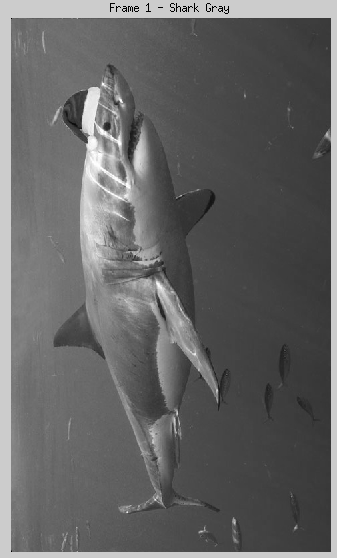
\includegraphics[scale=.5]{Images/DelayedThreshold/frame1.png}
&
  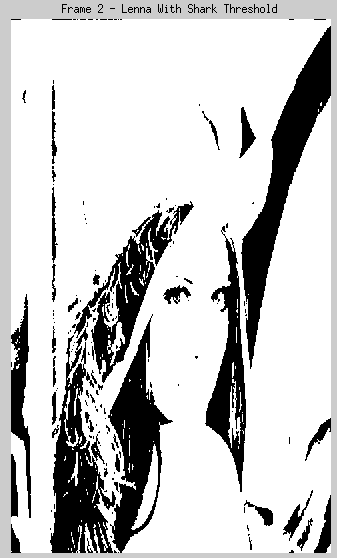
\includegraphics[scale=.5]{Images/DelayedThreshold/frame2.png}
&
  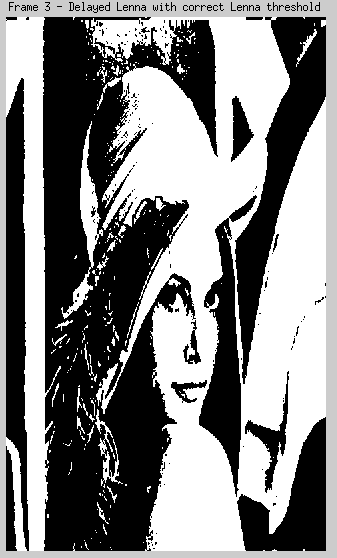
\includegraphics[scale=.5]{Images/DelayedThreshold/frame3.png}
\end{tabular}
\end{center}
\captionof{figure}{Frame 1: Shark warmup frame. Frame 2: Lenna thresholded with Shark threshold. Frame 3: Lenna frame delayed and thresholded correctly.}
\label{fig:lenna_thresh_shark}
\end{table}
  
\newpage
  \section{Appendix B - Signal Tap and Simulation Results}
  \subsection{Histogram}
    \begin{figure}[H]
    \centering{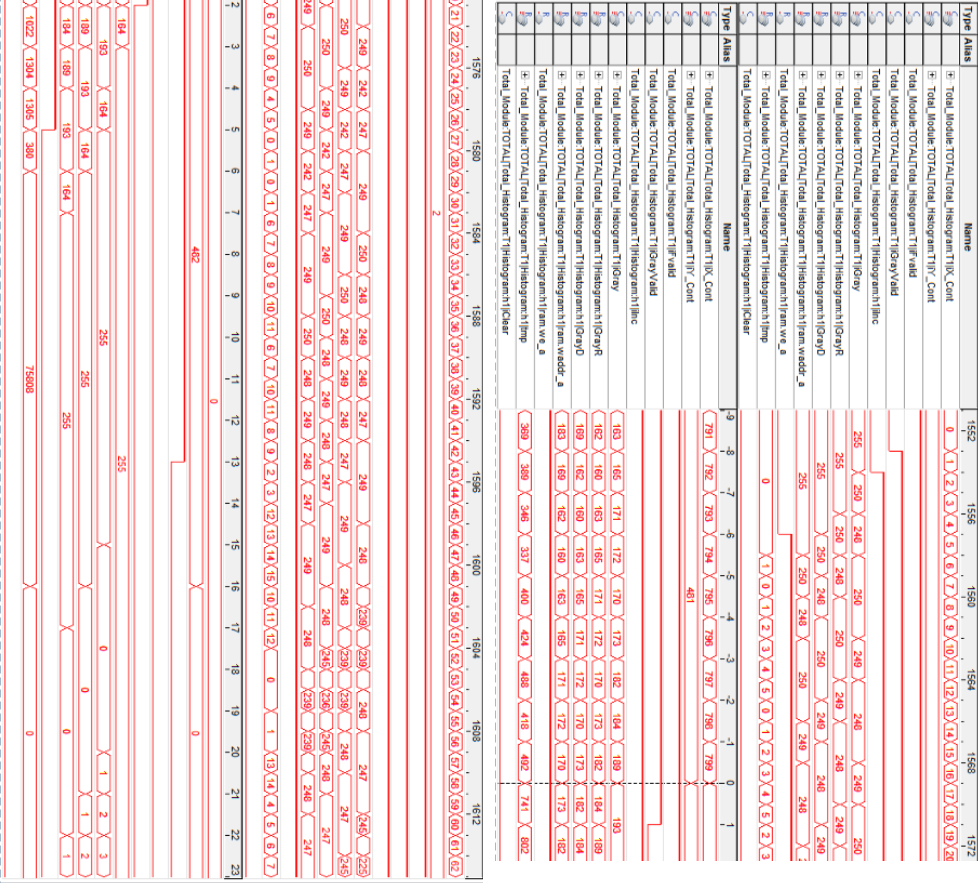
\includegraphics[width=\textwidth]{Images/NormalHistogram.png}}
    \caption{Normal Histogram Operation - Signal Tap}
    \label{fig:norm_hist}
  \end{figure}
  
  \begin{figure}[H]
    \centering{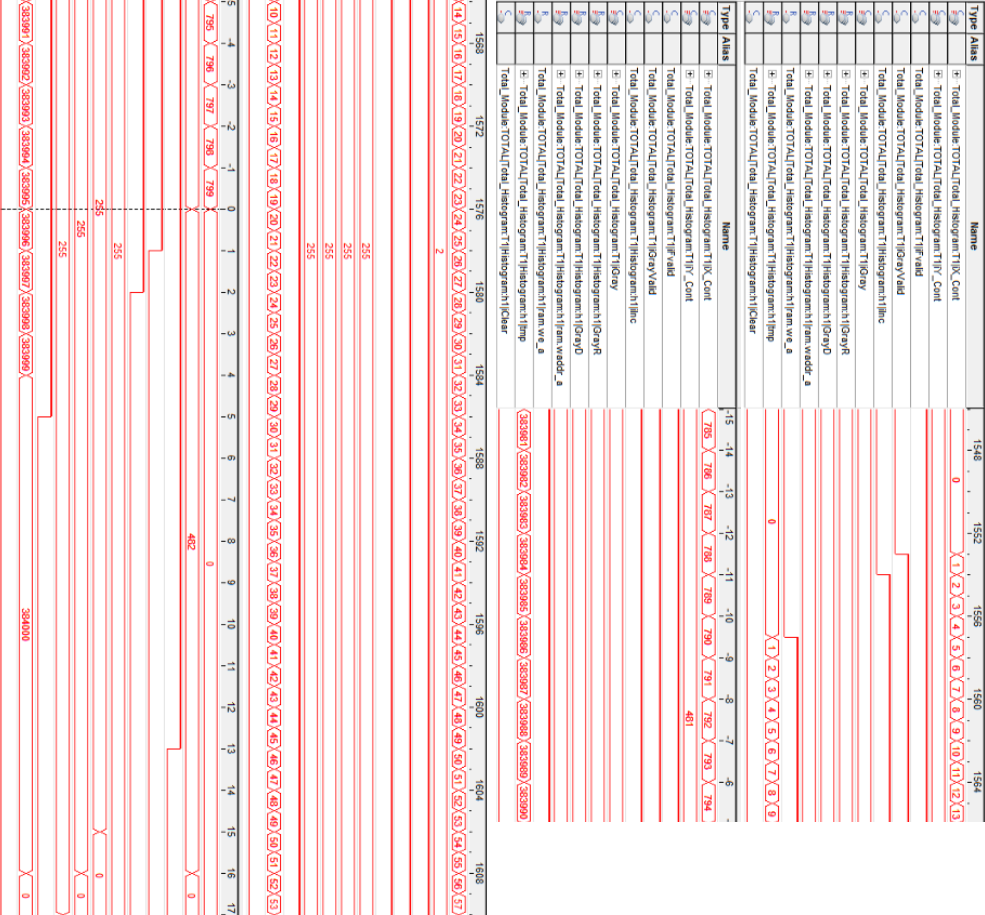
\includegraphics[width=\textwidth]{Images/EdgeCaseHistogram.png}}
    \caption{Edge Case Histogram Operation - Signal Tap}
    \label{fig:edge_hist}
  \end{figure}
  
    \begin{figure}[H]
    \centering{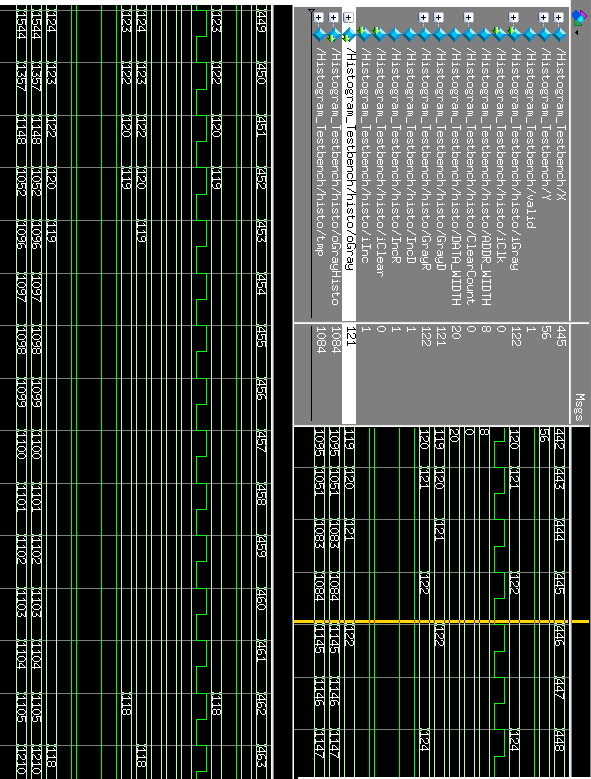
\includegraphics[width=\textwidth]{Images/ModelSimHistogram.png}}
    \caption{Histogram Operation - ModelSim}
    \label{fig:edge_histmod}
  \end{figure}
  \newpage
  \subsection{Cumulative Histogram}
    \begin{figure}[H]
    \centering{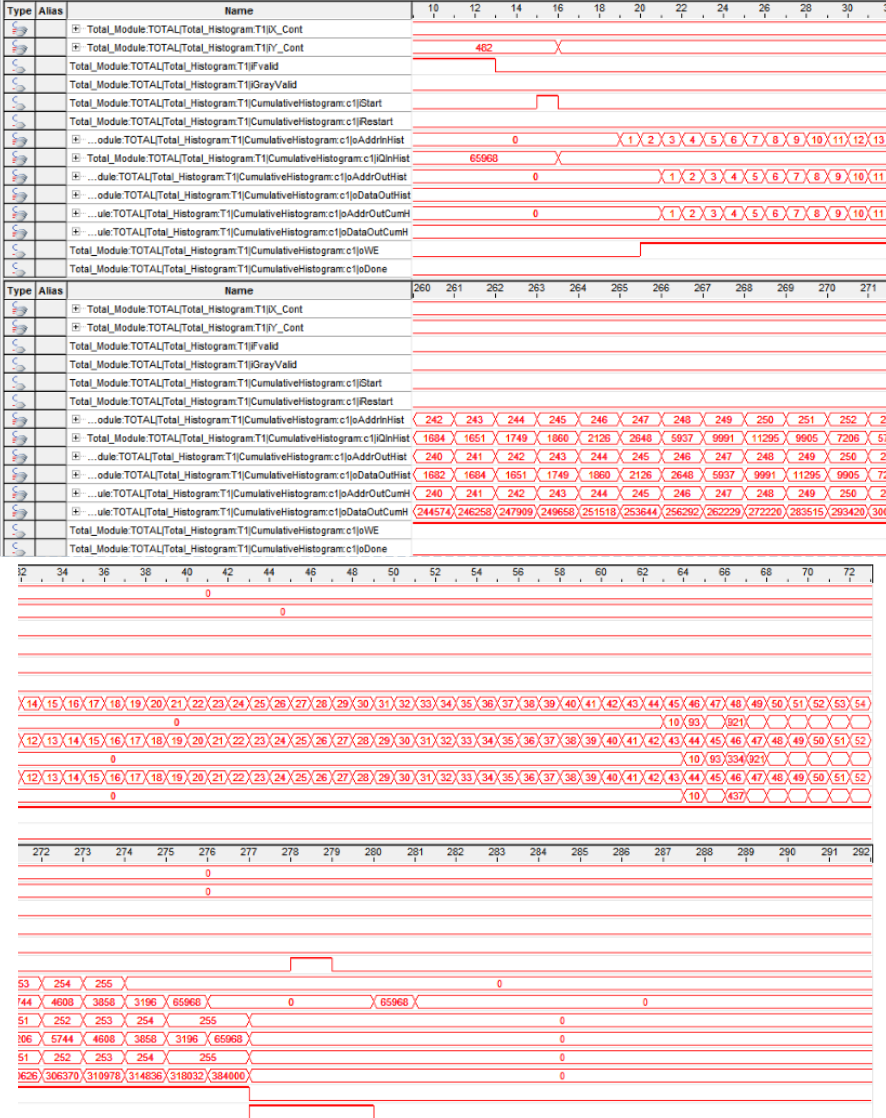
\includegraphics[width=\textwidth]{Images/NormalCumulative.png}}
    \caption{Cumulative Histogram Operation - Signal Tap}
    \label{fig:norm_histcum}
  \end{figure}
  
  \begin{figure}[H]
    \centering{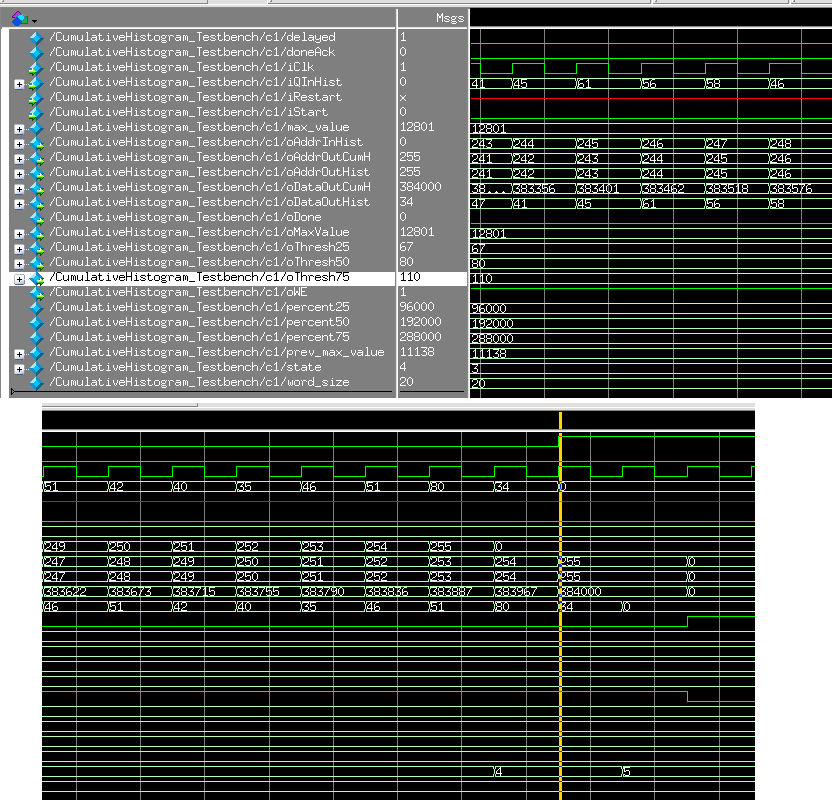
\includegraphics[width=\textwidth]{Images/ModelSimCumulative.png}}
    \caption{Cumulative Histogram Operation - ModelSim}
    \label{fig:nomr_modhist}
  \end{figure}
  
  \section{Appendix C - RTL Diagrams}
    \begin{figure}[H]
    \centering{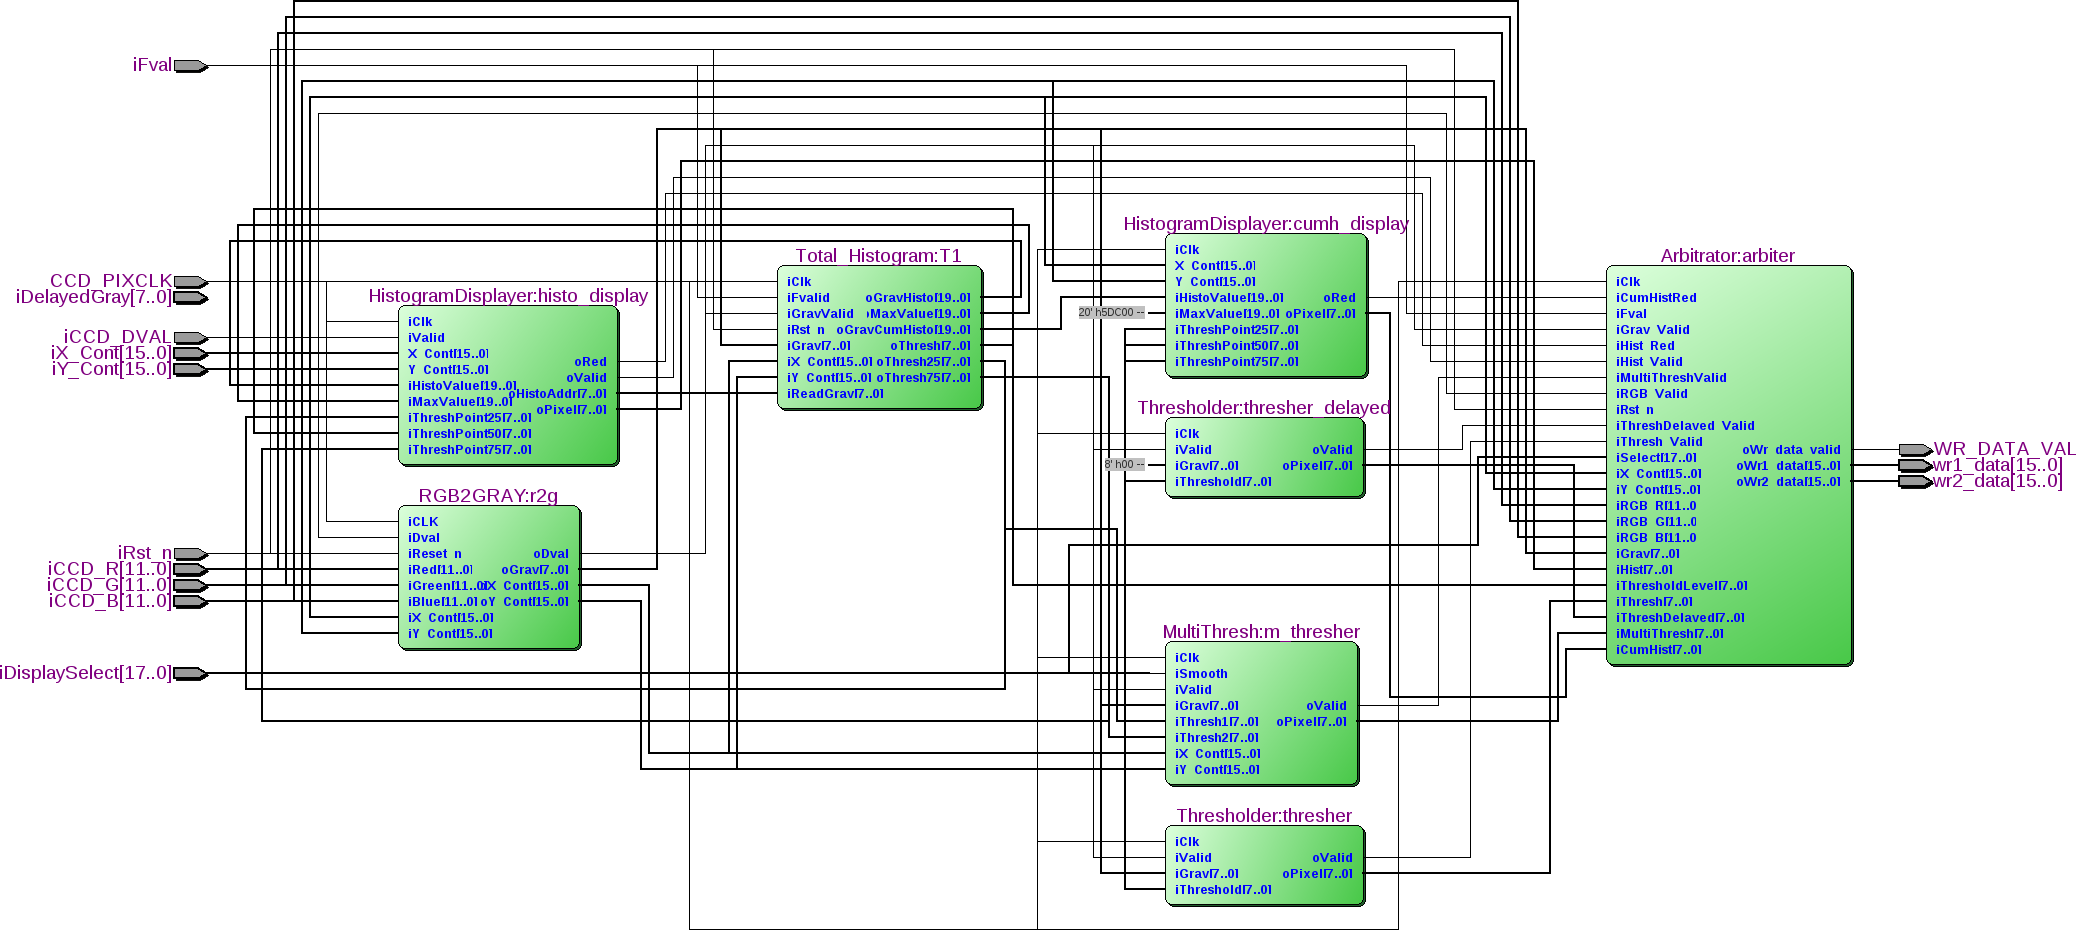
\includegraphics[width=\textwidth]{Images/Total_ModuleRTL.png}}
    \caption{Total\_Module RTL Diagram}
    \label{fig:nomr_modhissast}
  \end{figure}
  
  
    \begin{figure}[H]
    \centering{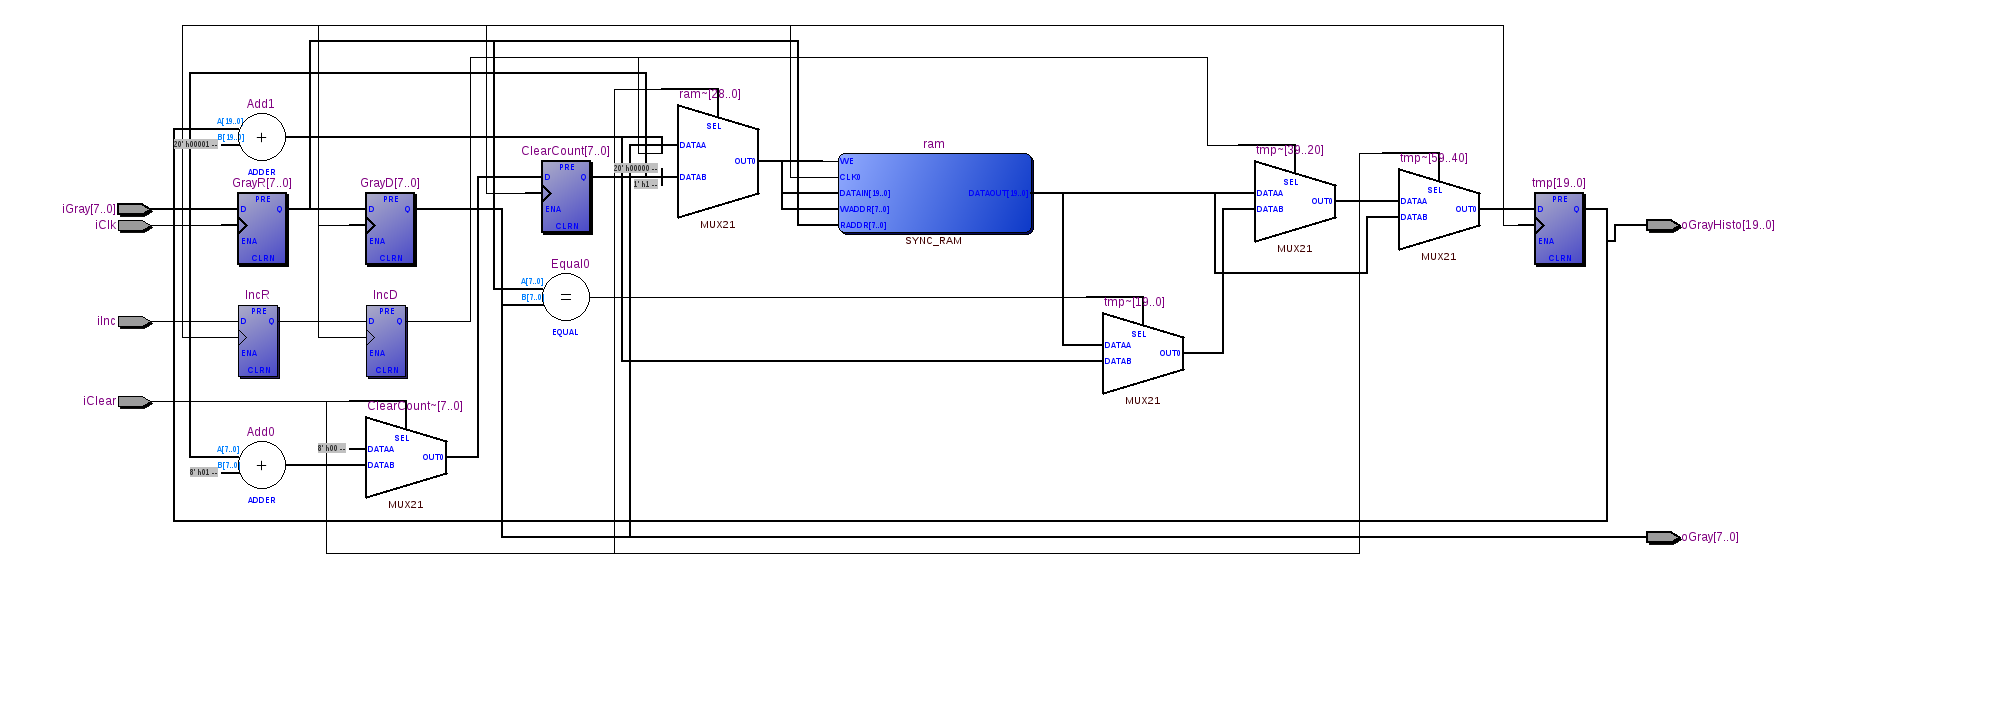
\includegraphics[width=\textwidth]{Images/HistogramRTL.png}}
    \caption{Histogram RTL Diagram}
    \label{fig:nomr_modhisrtt}
  \end{figure}
  
  
    \begin{figure}[H]
    \centering{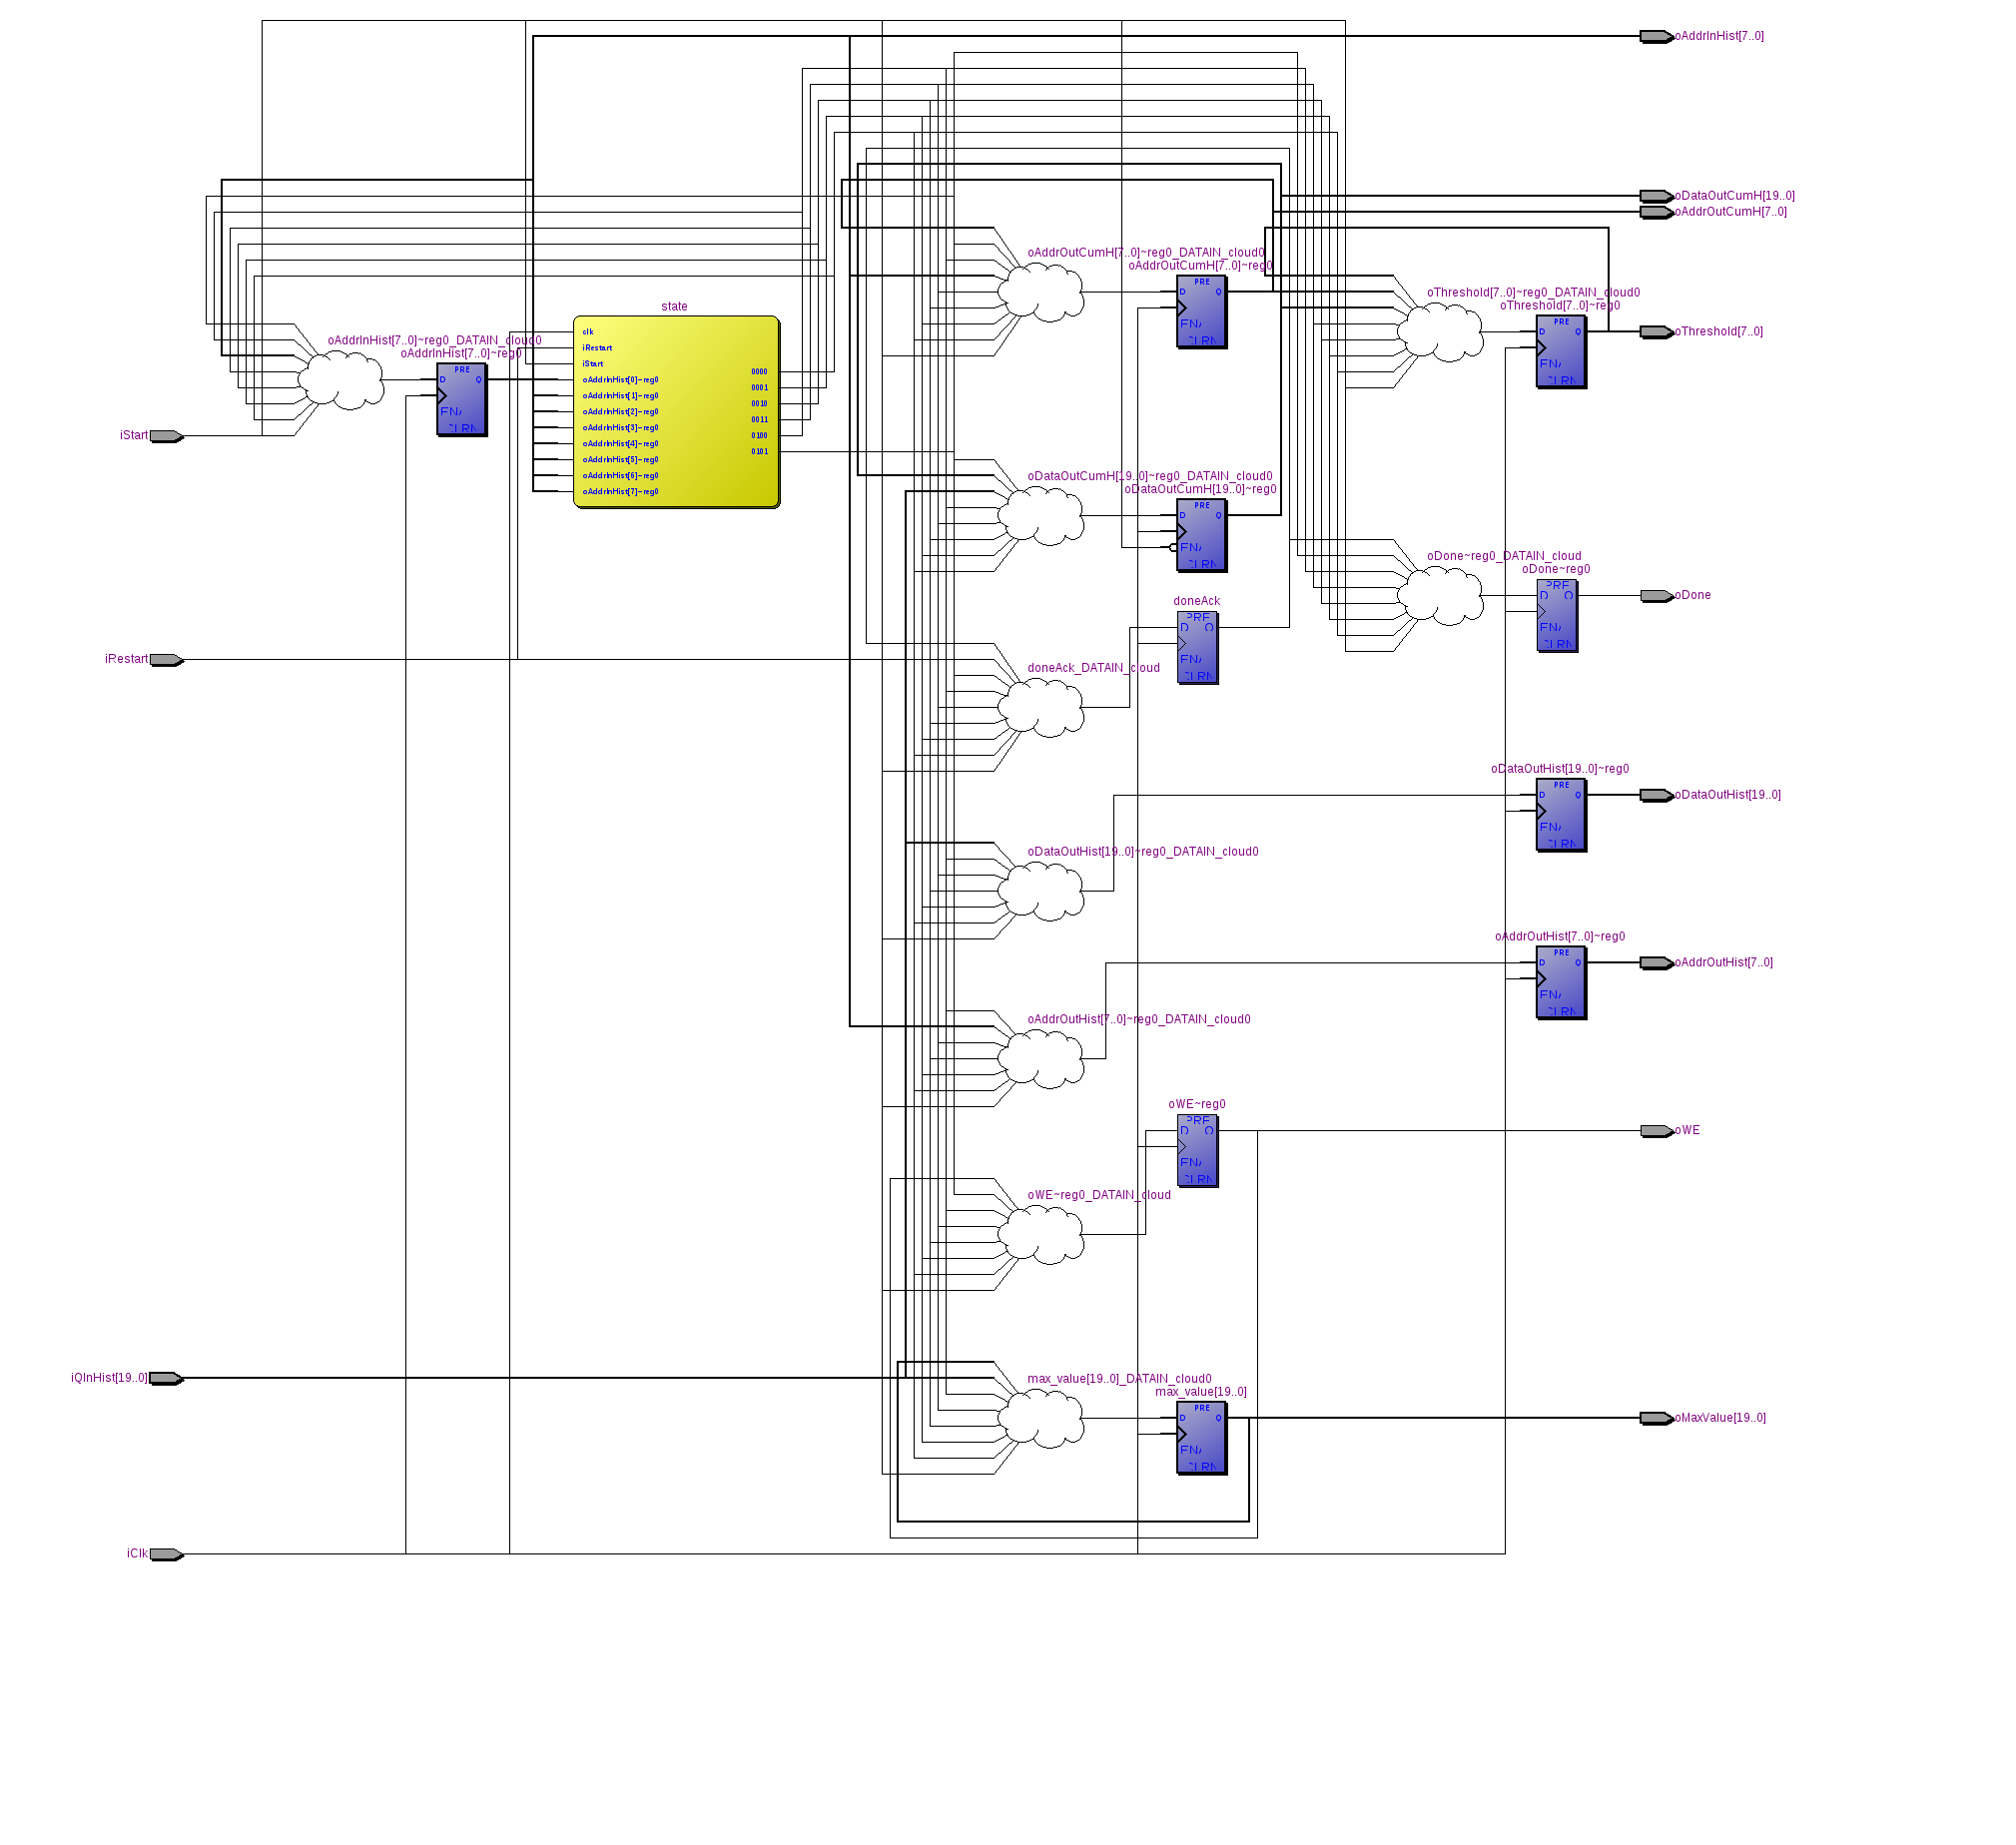
\includegraphics[width=\textwidth]{Images/CumulativeHistogramRTL.png}}
    \caption{Cumulative Histogram RTL Diagram}
    \label{fig:nomr_modhistrtlc}
  \end{figure}
  
  
    \begin{figure}[H]
    \centering{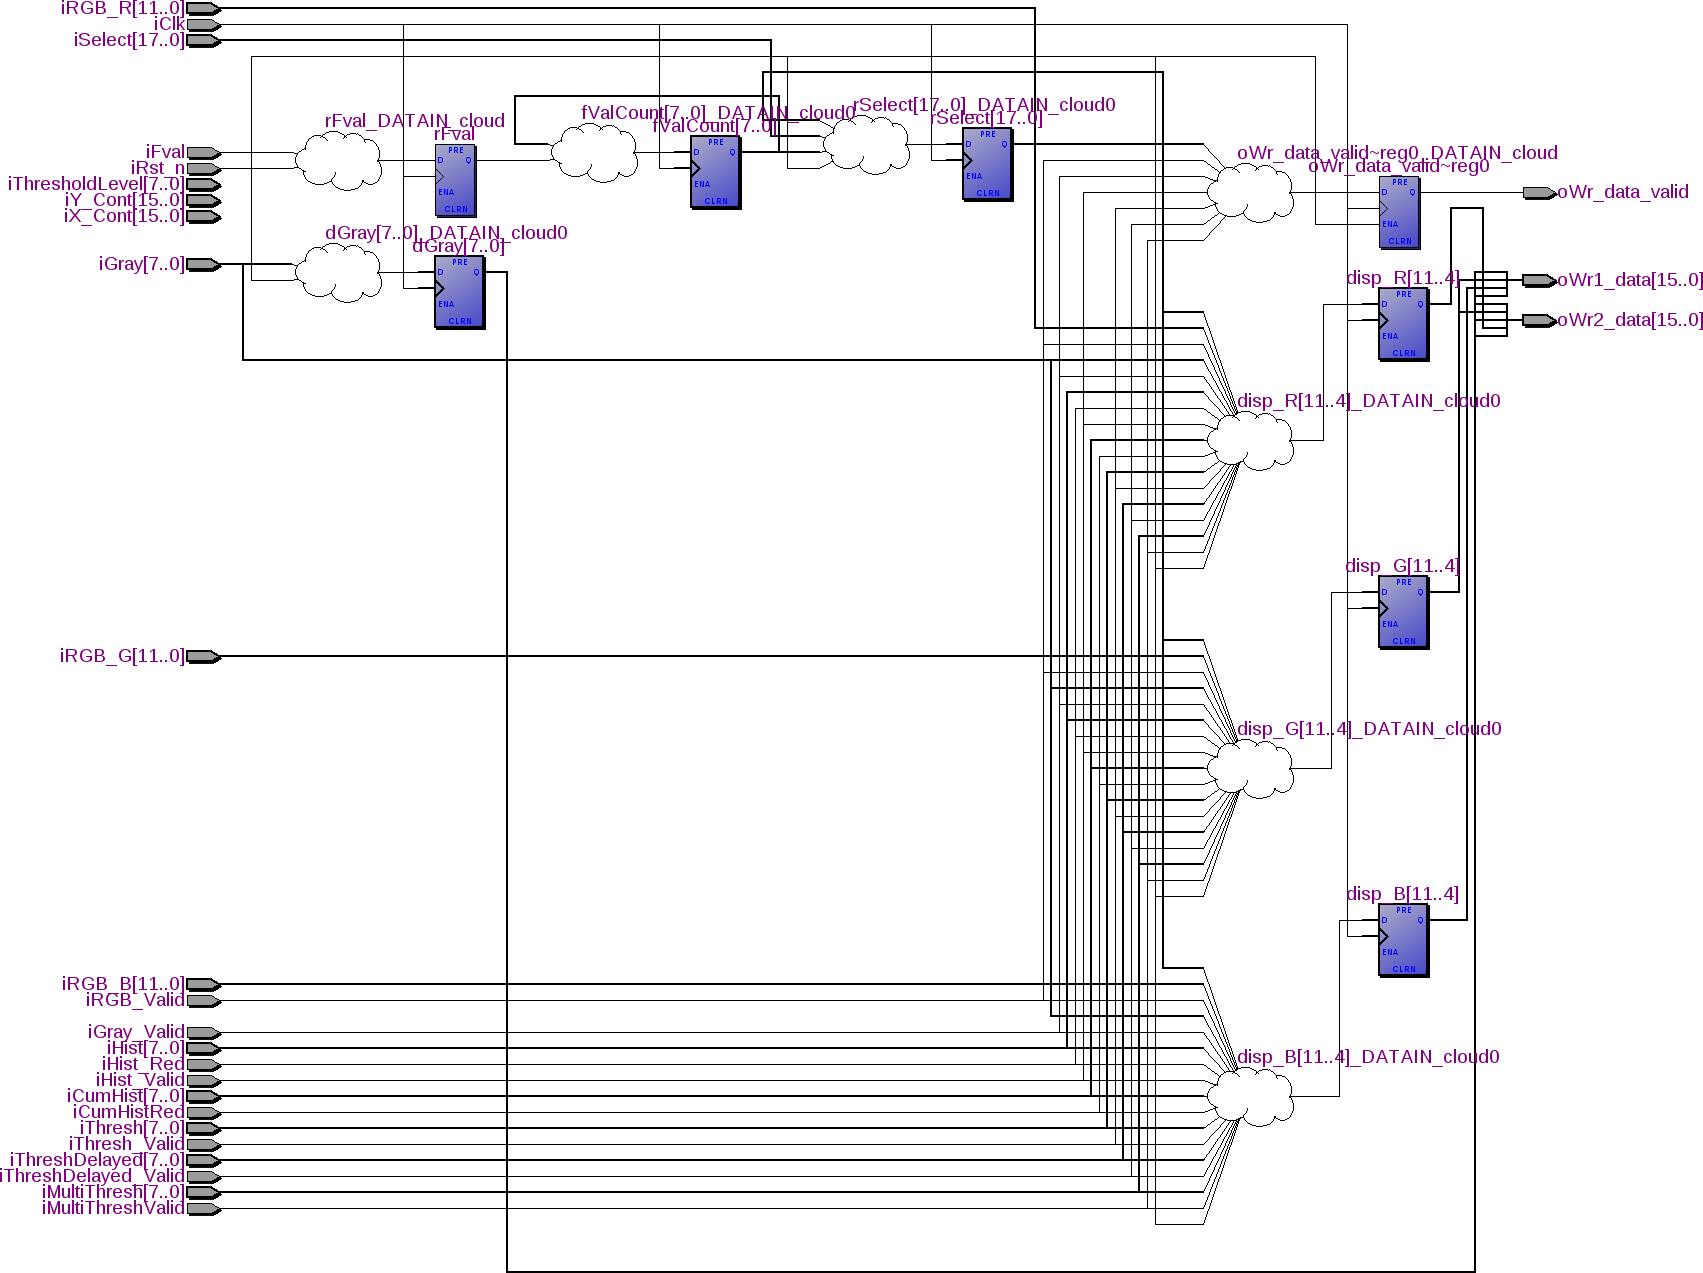
\includegraphics[width=\textwidth]{Images/ArbitratorRTL.png}}
    \caption{Arbitrator RTL Diagram}
    \label{fig:narobmr_modhist}
  \end{figure}
  
  
    \begin{figure}[H]
    \centering{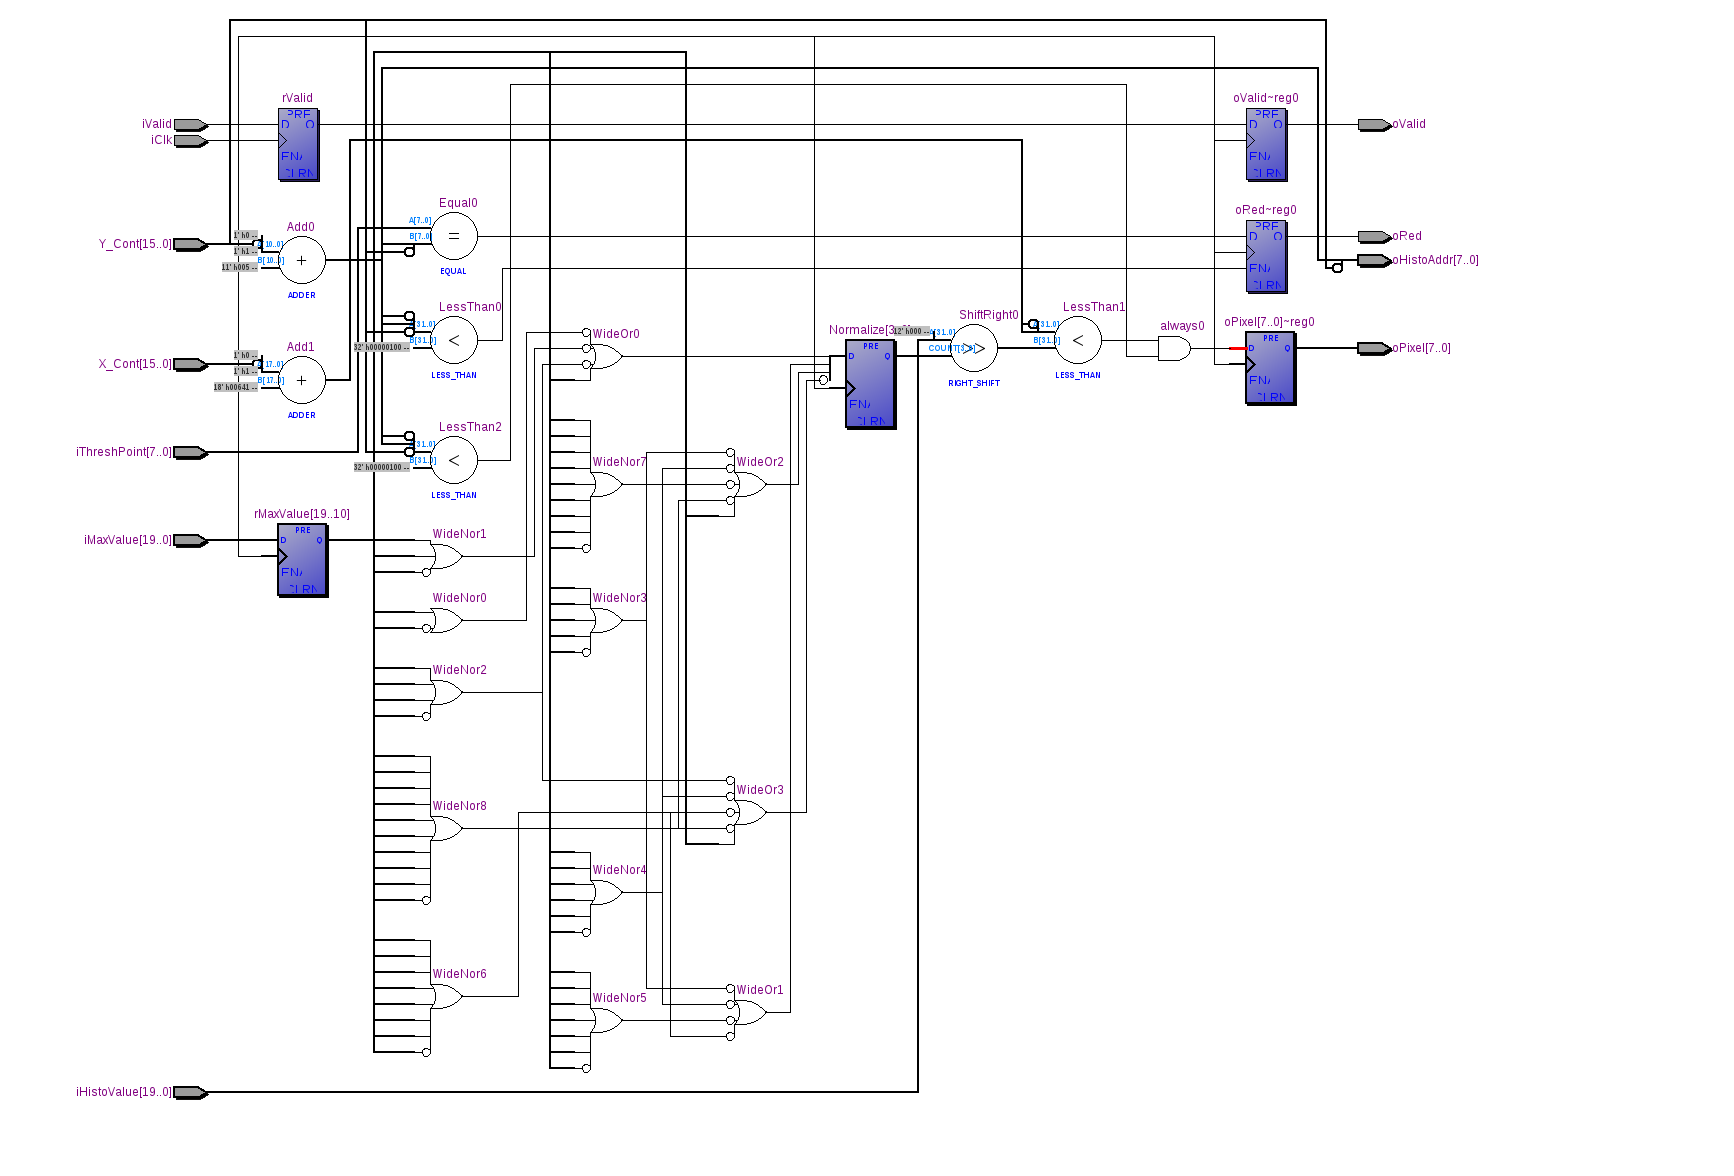
\includegraphics[width=\textwidth]{Images/HistogramDisplayerRTL.png}}
    \caption{Histogram Displayer RTL Diagram}
    \label{fig:nomr_modhist}
  \end{figure}
  
      \begin{figure}[H]
    \centering{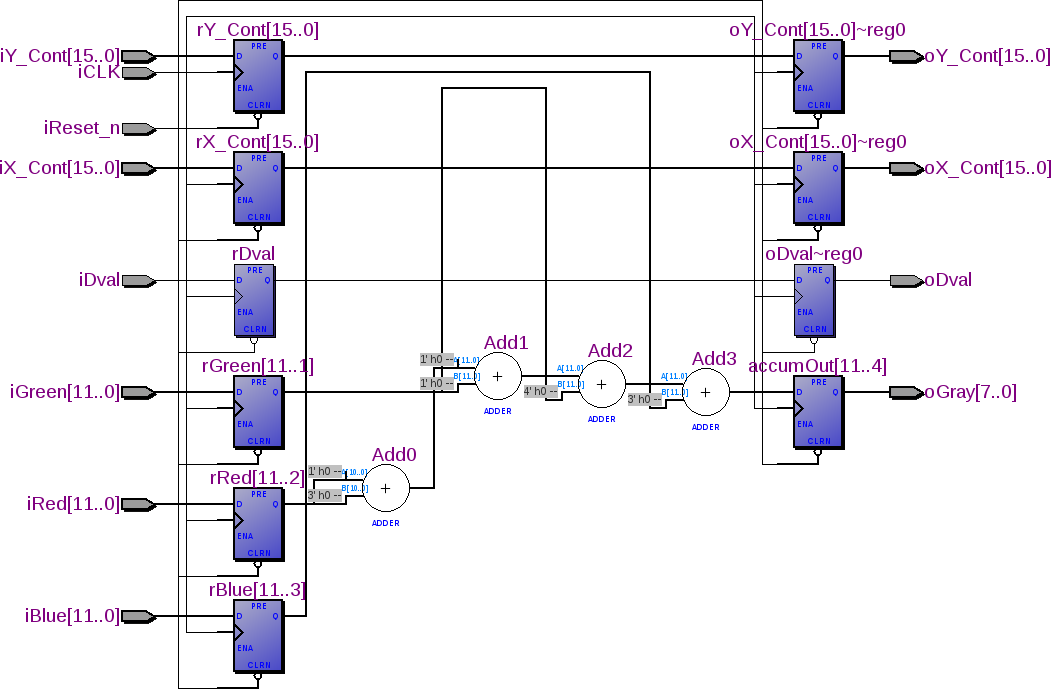
\includegraphics[width=\textwidth]{Images/RGB2GRAYRTL.png}}
    \caption{RGB2GRAY RTL Diagram}
    \label{fig:nomr_modhist}
  \end{figure}
  
        \begin{figure}[H]
    \centering{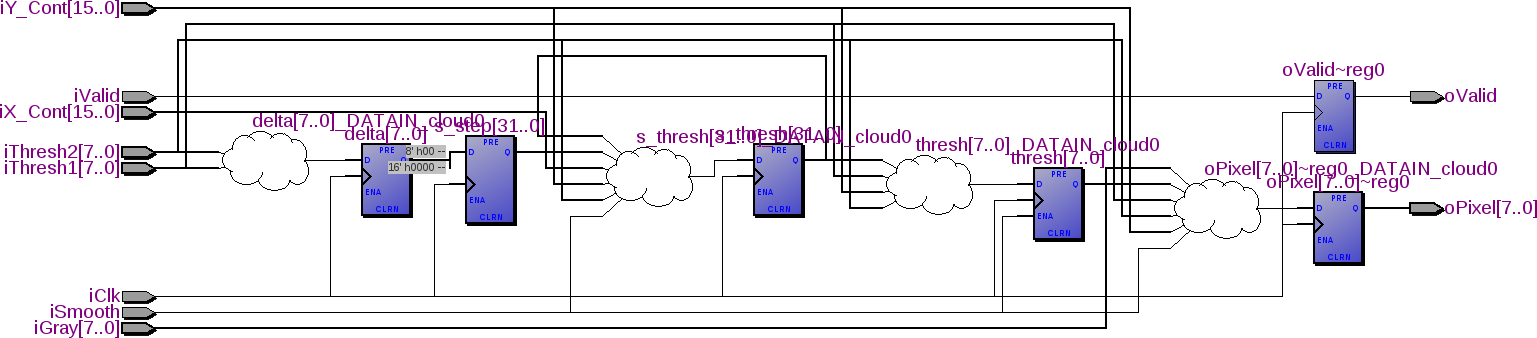
\includegraphics[width=\textwidth]{Images/MultiThreshRTL.png}}
    \caption{MultiThresh RTL Diagram}
    \label{fig:nomr_modhist}
  \end{figure}
  
  
  
\end{document}
